\documentclass[aspectratio=169]{beamer}
\usepackage[utf8]{inputenc}
\usepackage[T1]{fontenc}
\usepackage{svg}
\usepackage{todonotes}
\usepackage{siunitx}

\setbeamertemplate{caption}[numbered]

\title{Open Data: \\ Receive it Yourself}
\date[ISPN ’80]{Datenspuren 2022, Dresden}
\author[]{Tassilo, 0xA, Marenz (dump@dvb.solutions)}

\usetheme{dvb}

\AtBeginSection[]{
  \begingroup
  \setbeamertemplate{background}{
    \begin{tikzpicture}
      \useasboundingbox (0,0) rectangle(\the\paperwidth,\the\paperheight);
      \fill[dvbyellow,rotate around={70:(0,0)}] (0,-2) rectangle (22,0);
      \fill[dvbyellow,rotate around={70:(3,0)}] (0,-2) rectangle (22,0);
    \end{tikzpicture}
  }
  \begin{frame}
  \vskip4cm%
    \begin{beamercolorbox}[wd=12cm,leftskip=3cm]{title page header}
    	\usebeamerfont{title}\textbf{\LARGE \fontfamily{pag}\selectfont \secname}\par%
    \end{beamercolorbox}
  \vfill
  \end{frame}
  \endgroup
}

\newcommand*{\myfont}{\fontfamily{pag}\selectfont}

\makeatletter
\tikzset{
    database/.style={
        path picture={
            \draw (0, 1.5*\database@segmentheight) circle [x radius=\database@radius,y radius=\database@aspectratio*\database@radius];
            \draw (-\database@radius, 0.5*\database@segmentheight) arc [start angle=180,end angle=360,x radius=\database@radius, y radius=\database@aspectratio*\database@radius];
            \draw (-\database@radius,-0.5*\database@segmentheight) arc [start angle=180,end angle=360,x radius=\database@radius, y radius=\database@aspectratio*\database@radius];
            \draw (-\database@radius,1.5*\database@segmentheight) -- ++(0,-3*\database@segmentheight) arc [start angle=180,end angle=360,x radius=\database@radius, y radius=\database@aspectratio*\database@radius] -- ++(0,3*\database@segmentheight);
        },
        minimum width=2*\database@radius + \pgflinewidth,
        minimum height=3*\database@segmentheight + 2*\database@aspectratio*\database@radius + \pgflinewidth,
    },
    database segment height/.store in=\database@segmentheight,
    database radius/.store in=\database@radius,
    database aspect ratio/.store in=\database@aspectratio,
    database segment height=0.1cm,
    database radius=0.25cm,
    database aspect ratio=0.35,
}
\makeatother

\begin{document}

\begin{frame}\titlepage
\end{frame}
  
\begin{frame} 
 %\includesvg{dvbdump}
\frametitle{Roadmap} 
%\framesubtitle{The proof uses \textit{reductio ad absurdum}.} 

\tableofcontents

\end{frame}

% =================================================

\begin{frame}
\frametitle{Protocol}
\framesubtitle{Protocolls used in different cities}
\begin{figure}
\centering
\missingfigure[figwidth=7cm]{}
\caption{Missing figure caption}
\end{figure}
\end{frame}

% =================================================

\section{Radio \& VDV 420}

% =================================================

\begin{frame}
\frametitle{Data sources}
\framesubtitle{Overview of traffic light control (Ampelbeeinflussung)}
\begin{figure}
\centering
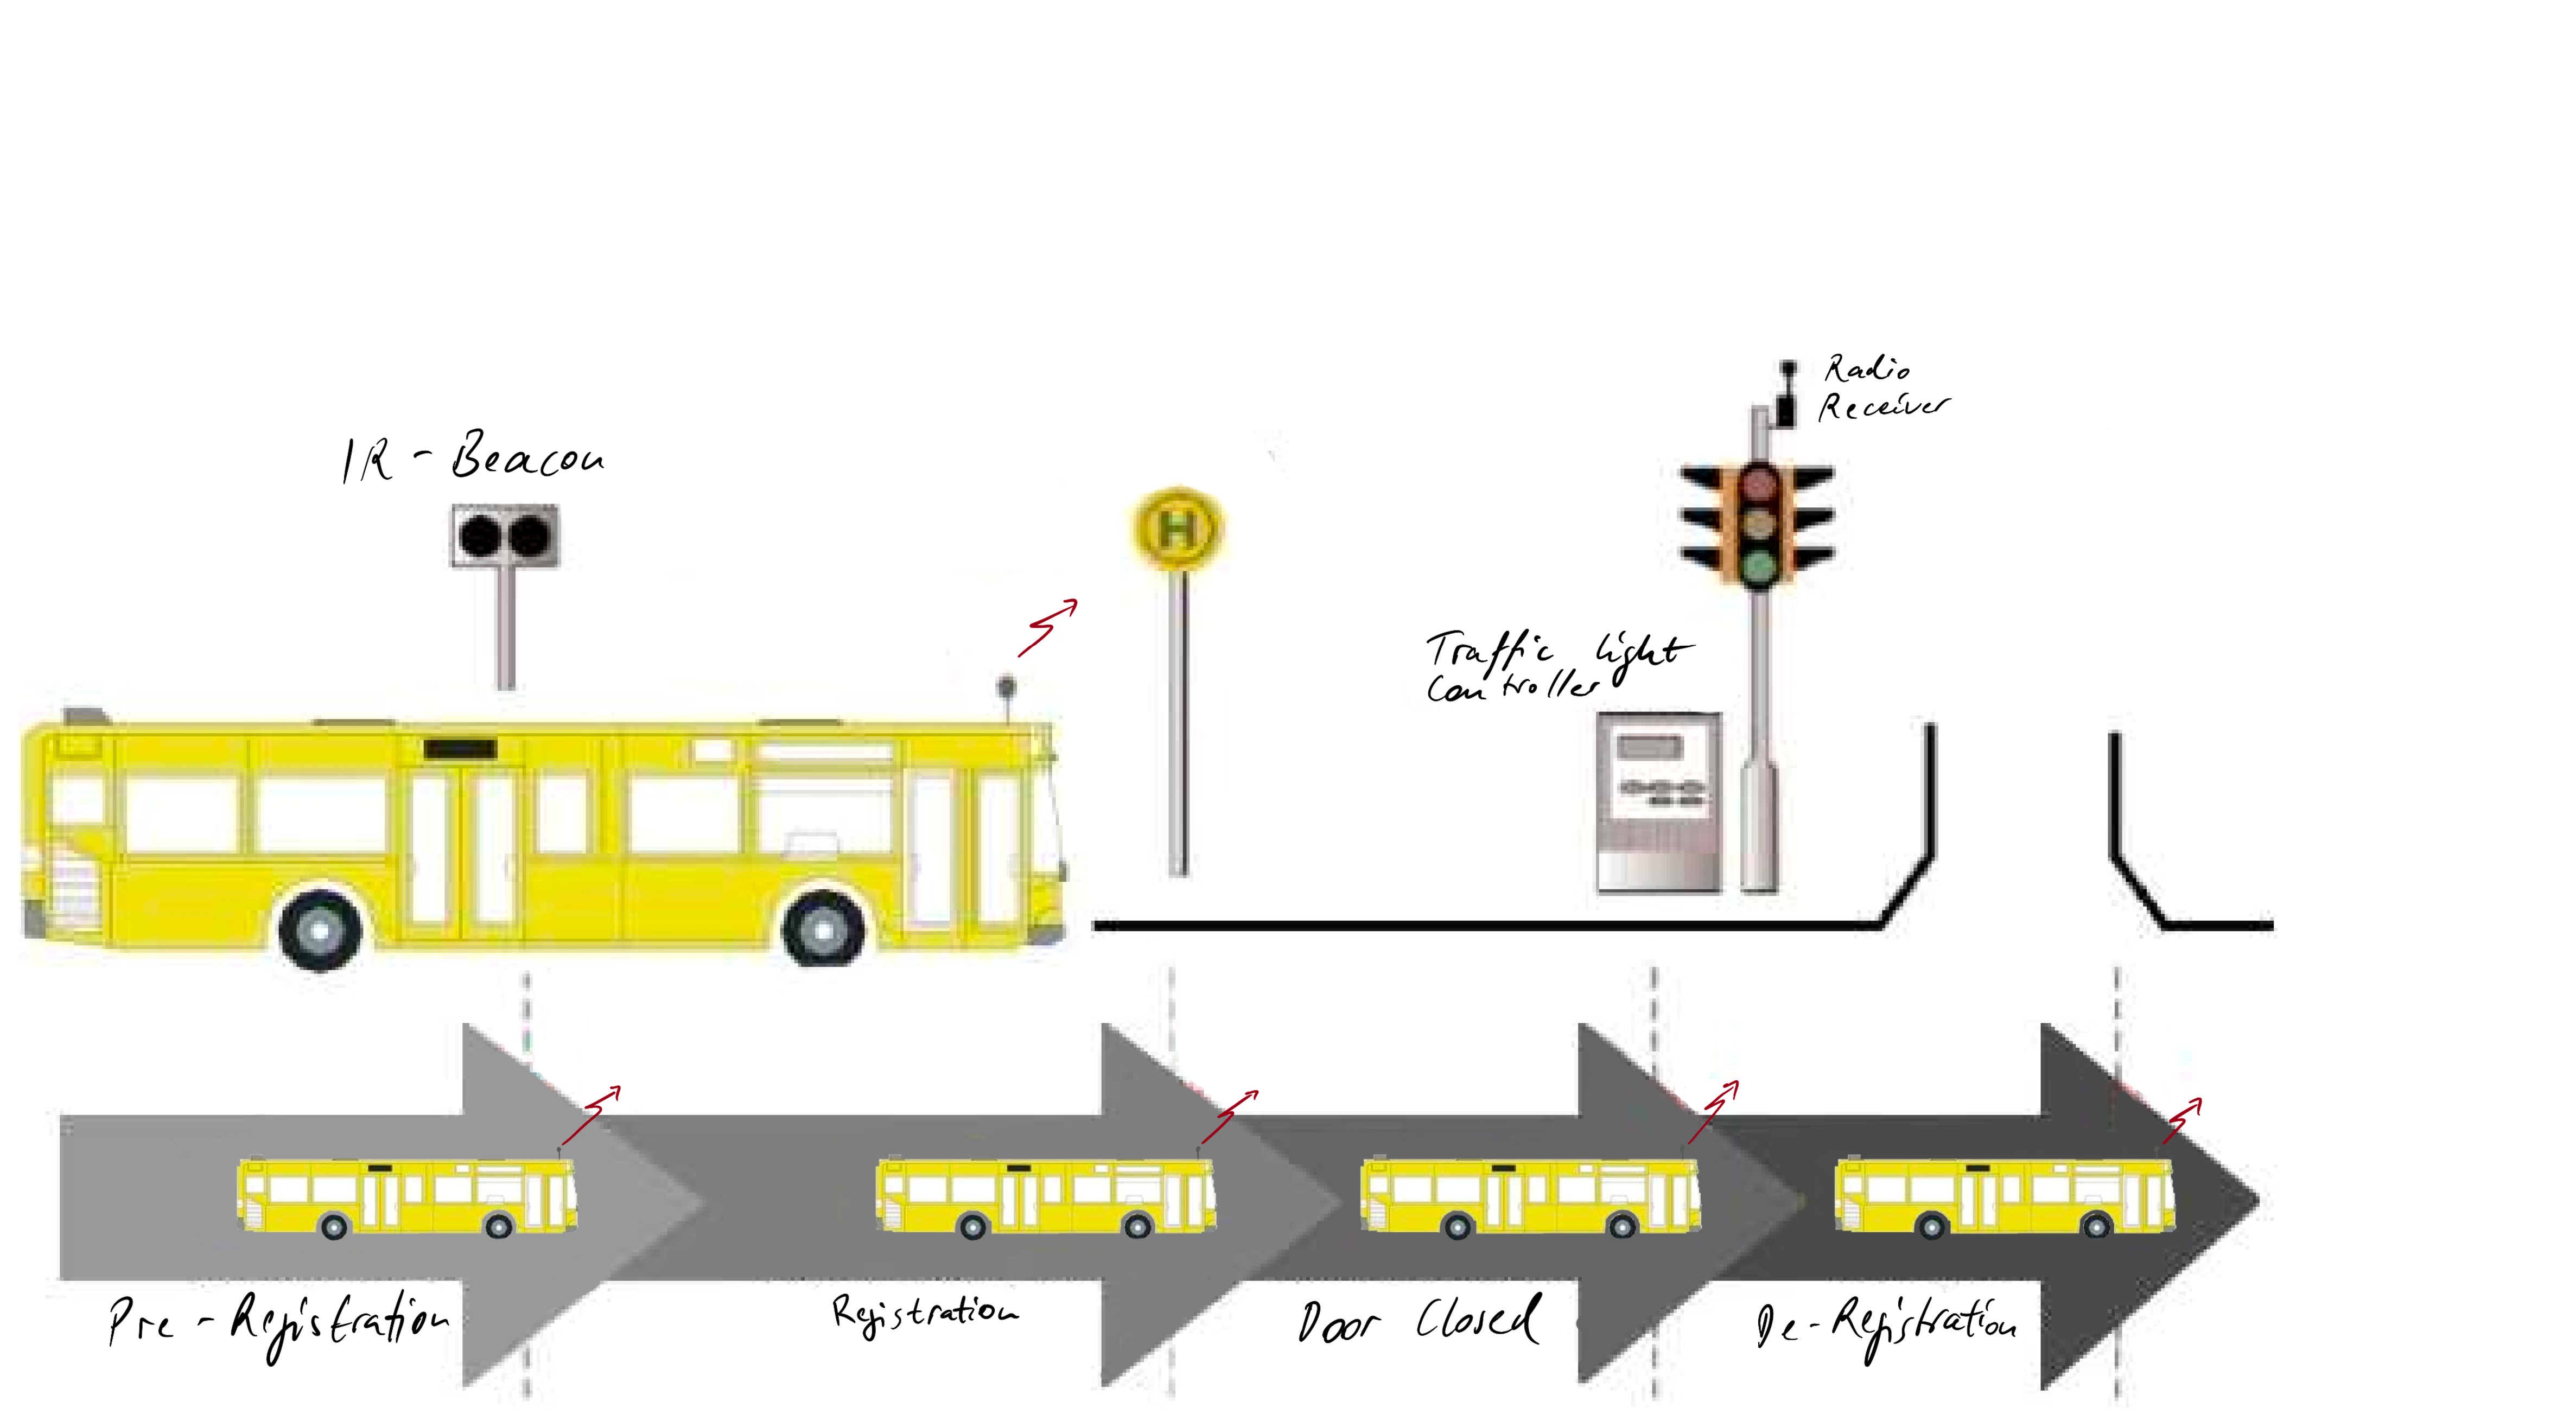
\includegraphics[height=0.65\textheight]{figs/lsa-beeinflussungs-stecke.pdf}
\caption{Traffic light controlled by radio link of busses and trams}
\end{figure}
\end{frame}

% =================================================

\begin{frame}
\frametitle{Data sources}
\framesubtitle{Overview of traffic light control (Ampelbeeinflussung)}
\begin{figure}
\centering
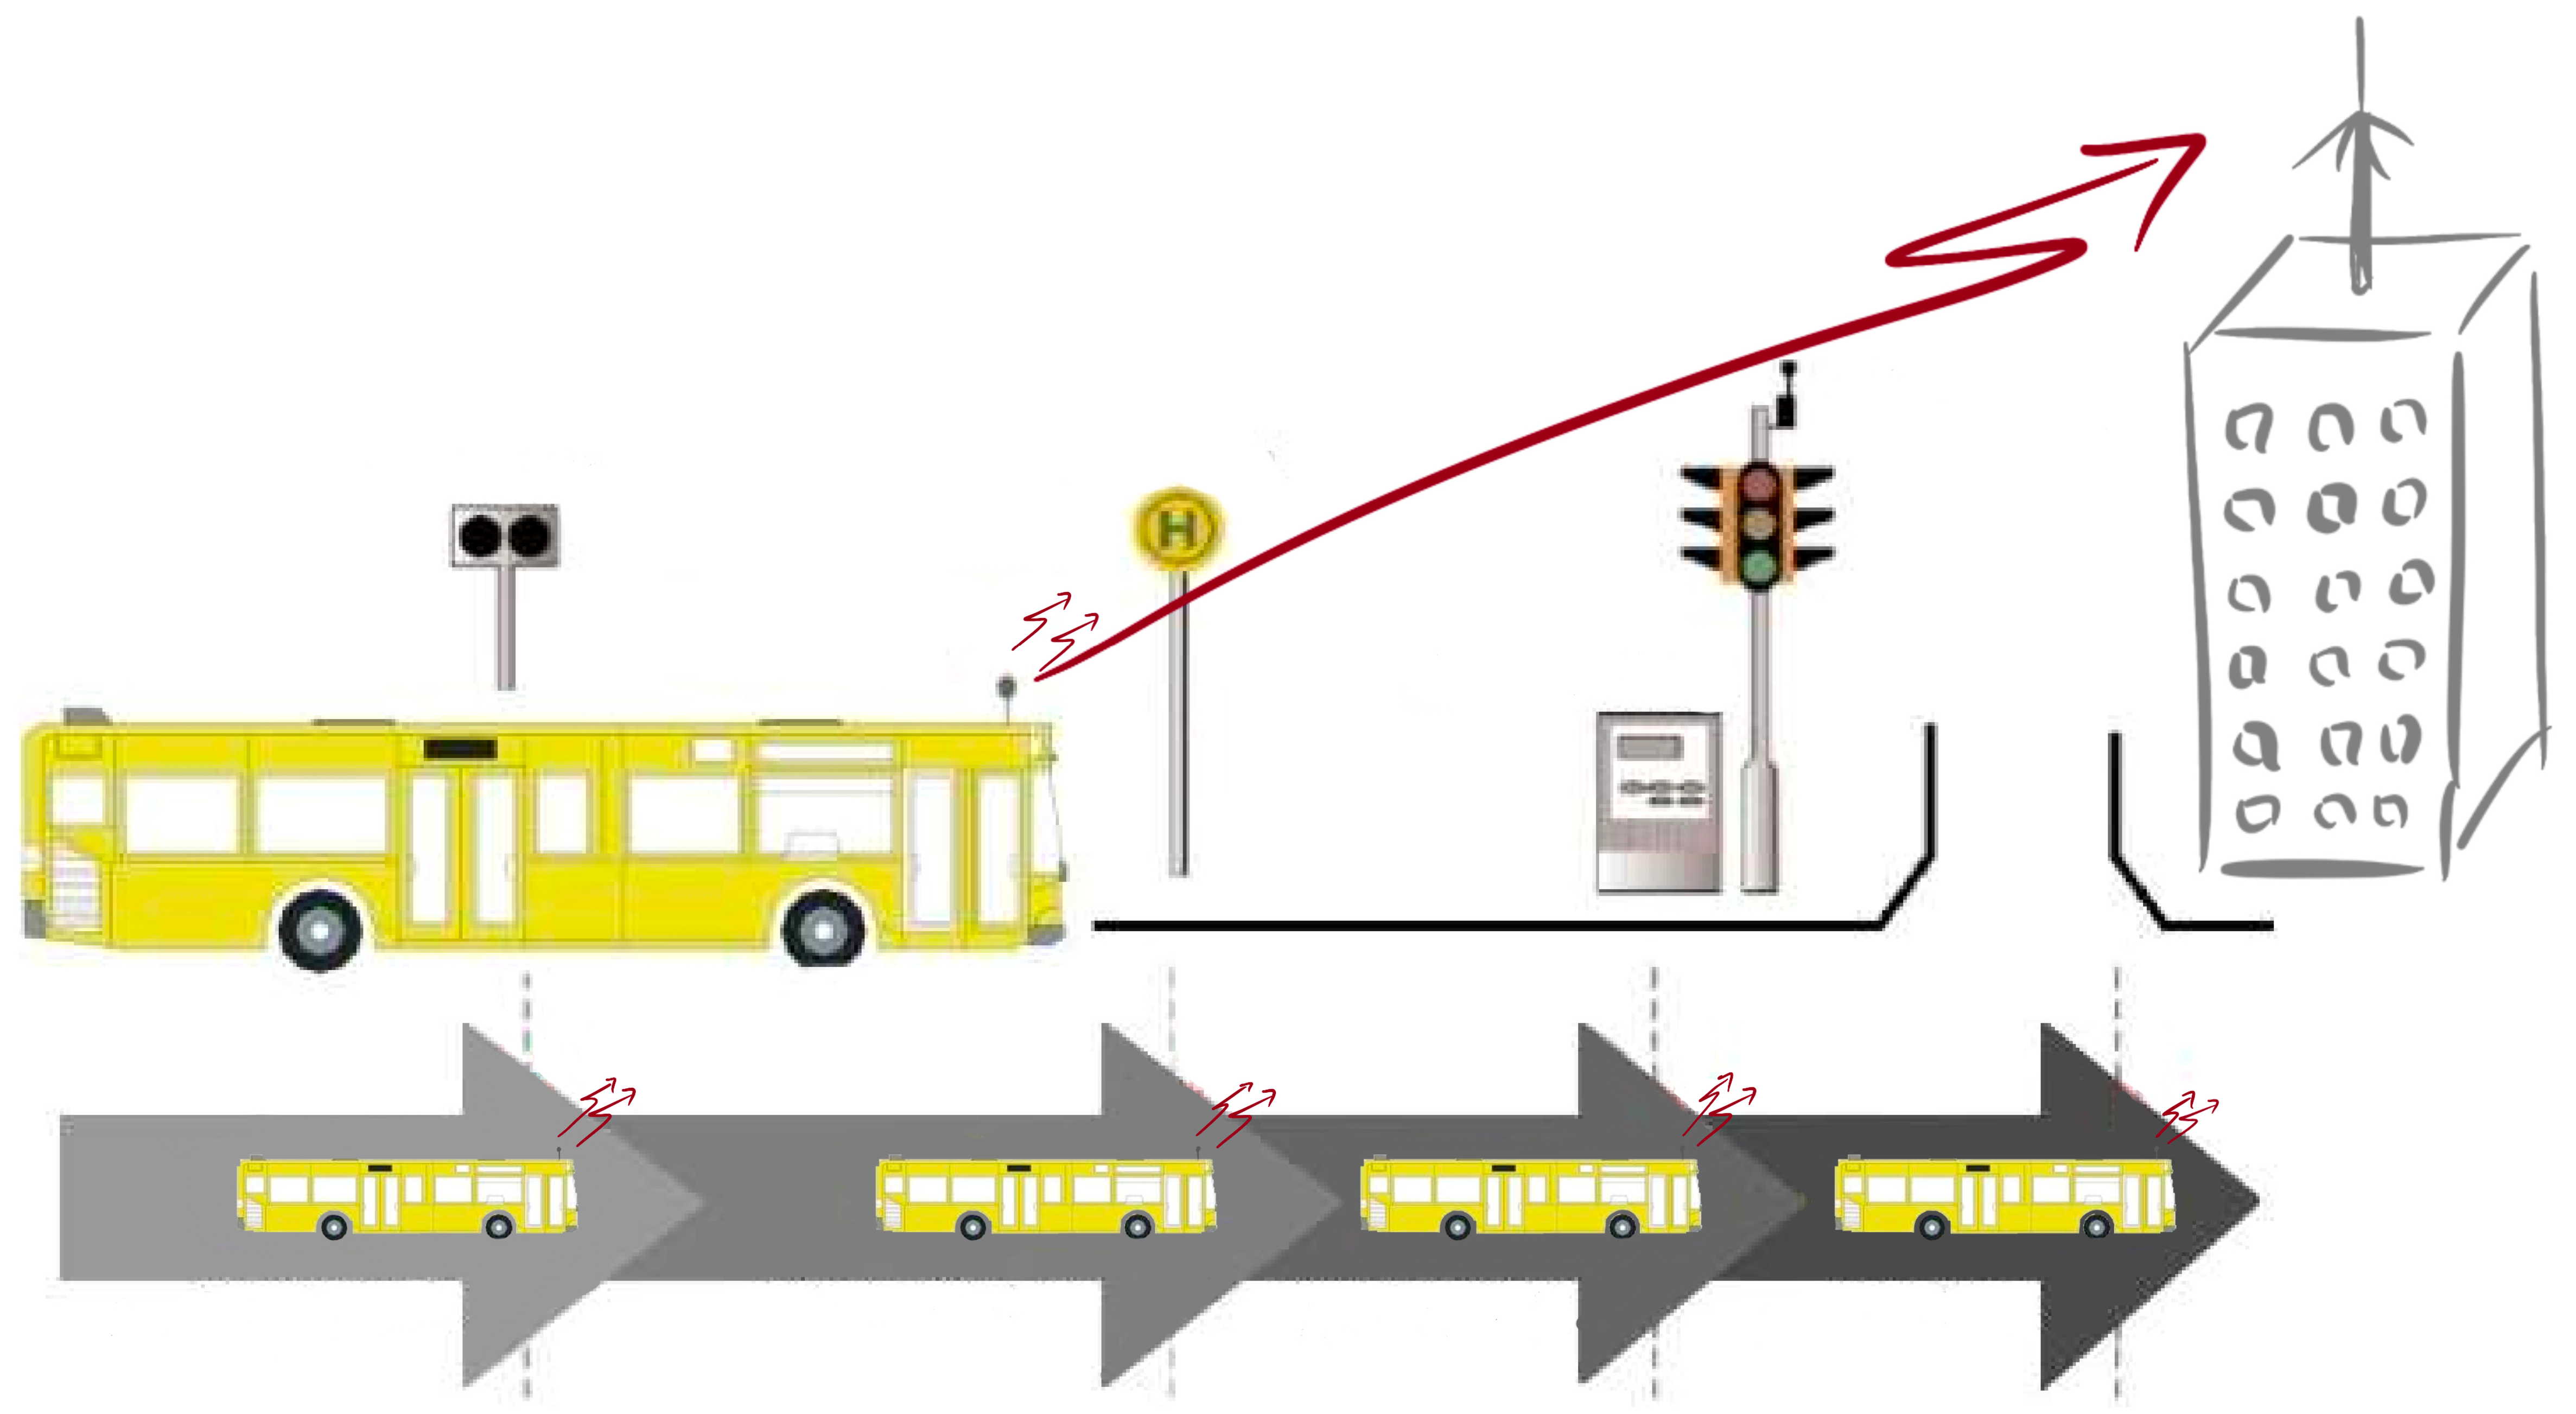
\includegraphics[height=0.65\textheight]{figs/lsa-beeinflussungs-stecke-mit-antenne.pdf}
\caption{Radio signals can be received by our antennas}
\end{figure}
\end{frame}

% =================================================

\begin{frame}
\frametitle{Data sources}
\framesubtitle{Receiver overview}
\begin{figure}
\centering
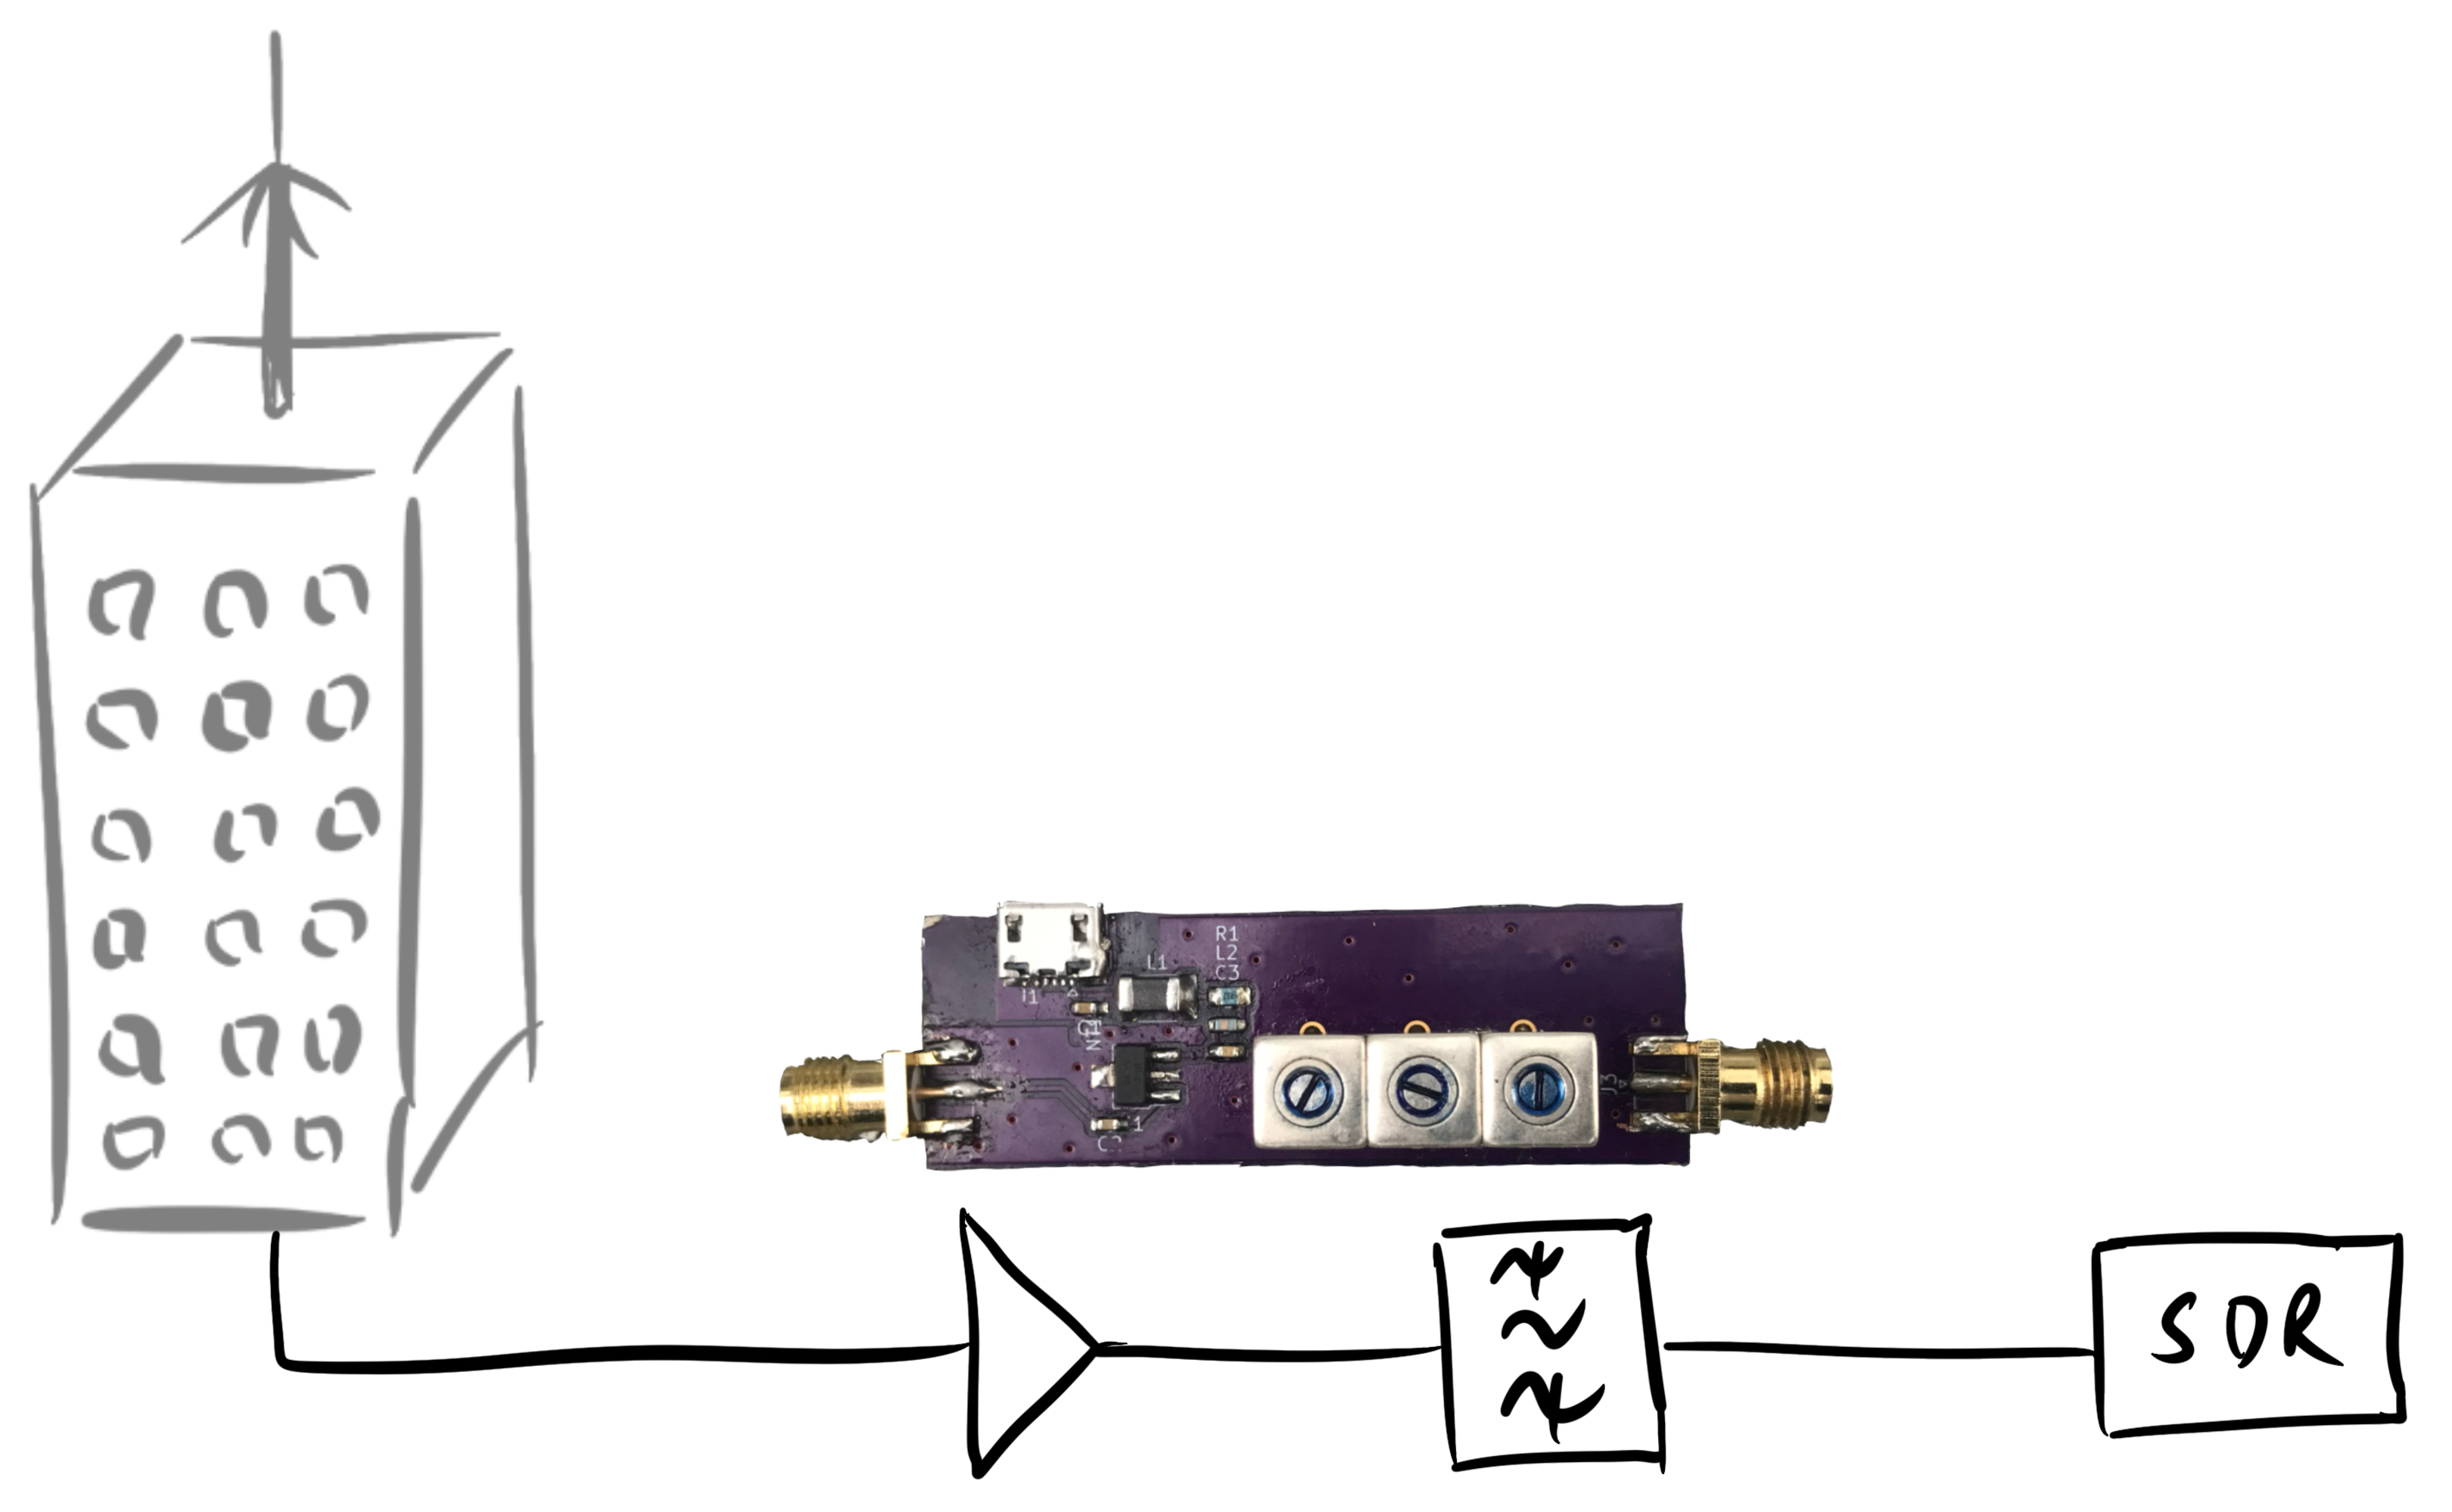
\includegraphics[height=0.65\textheight]{figs/antenna-filter.pdf}
\caption{Schematic overview of the receiver hardware}
\end{figure}
\end{frame}

% =================================================

\begin{frame}
\frametitle{Protocol}
\framesubtitle{VDV 420}
	\begin{itemize}
		\item which protocol?
		\item which frequency?
		\item some background on Ampelbeeinflussung and VDV 420 / 426
		\item R09 telegrams of trams and busses standardized in \href{https://knowhow.vdv.de/documents/420/}{VDV 420}
	\end{itemize}
\end{frame}

% =================================================

\begin{frame}
\title{test}
%\frametitle{Protocol}
%\framesubtitle{VDV 420 data}
\begin{itemize}
	\item what data can we receive?
	\begin{itemize}
		\item Tram identification data: line number, run number, destination number
		\item Location data: traffic light id, direction, registration\_type
		\item and some other (delay)
	\end{itemize}
\end{itemize}
\end{frame}

% =================================================

\begin{frame}
\frametitle{Protocol}
\framesubtitle{VDV 420 physical layer}
\begin{itemize}
	\item Minimum Shift Keying with \SI{2400}{Baud}
	\item bursty packet transmittion
		\item what frequency?
		\begin{itemize}
			\item look at the range of frequencies of RBL380, TODO add ranges
			\item take a look at our table, TODO link
			\item osint
		\end{itemize}
\end{itemize}
\end{frame}

% =================================================

\begin{frame}
\frametitle{Protocol}
\framesubtitle{Frequency identification}
\begin{figure}
\centering
\missingfigure[figwidth=7cm]{}
\caption{Screenshot of the bursty transmittion pattern}
\end{figure}
\end{frame}

% =================================================

\begin{frame}
\frametitle{Protocol}
\framesubtitle{Physical layer used in different cities}
\begin{figure}
% https://opus4.hbz-nrw.de/opus45-bast/frontdoor/deliver/index/docId/2595/file/V353+BF+Gesamtversion.pdf
% page 25
\begin{columns}
\column{.5\linewidth}
\centering
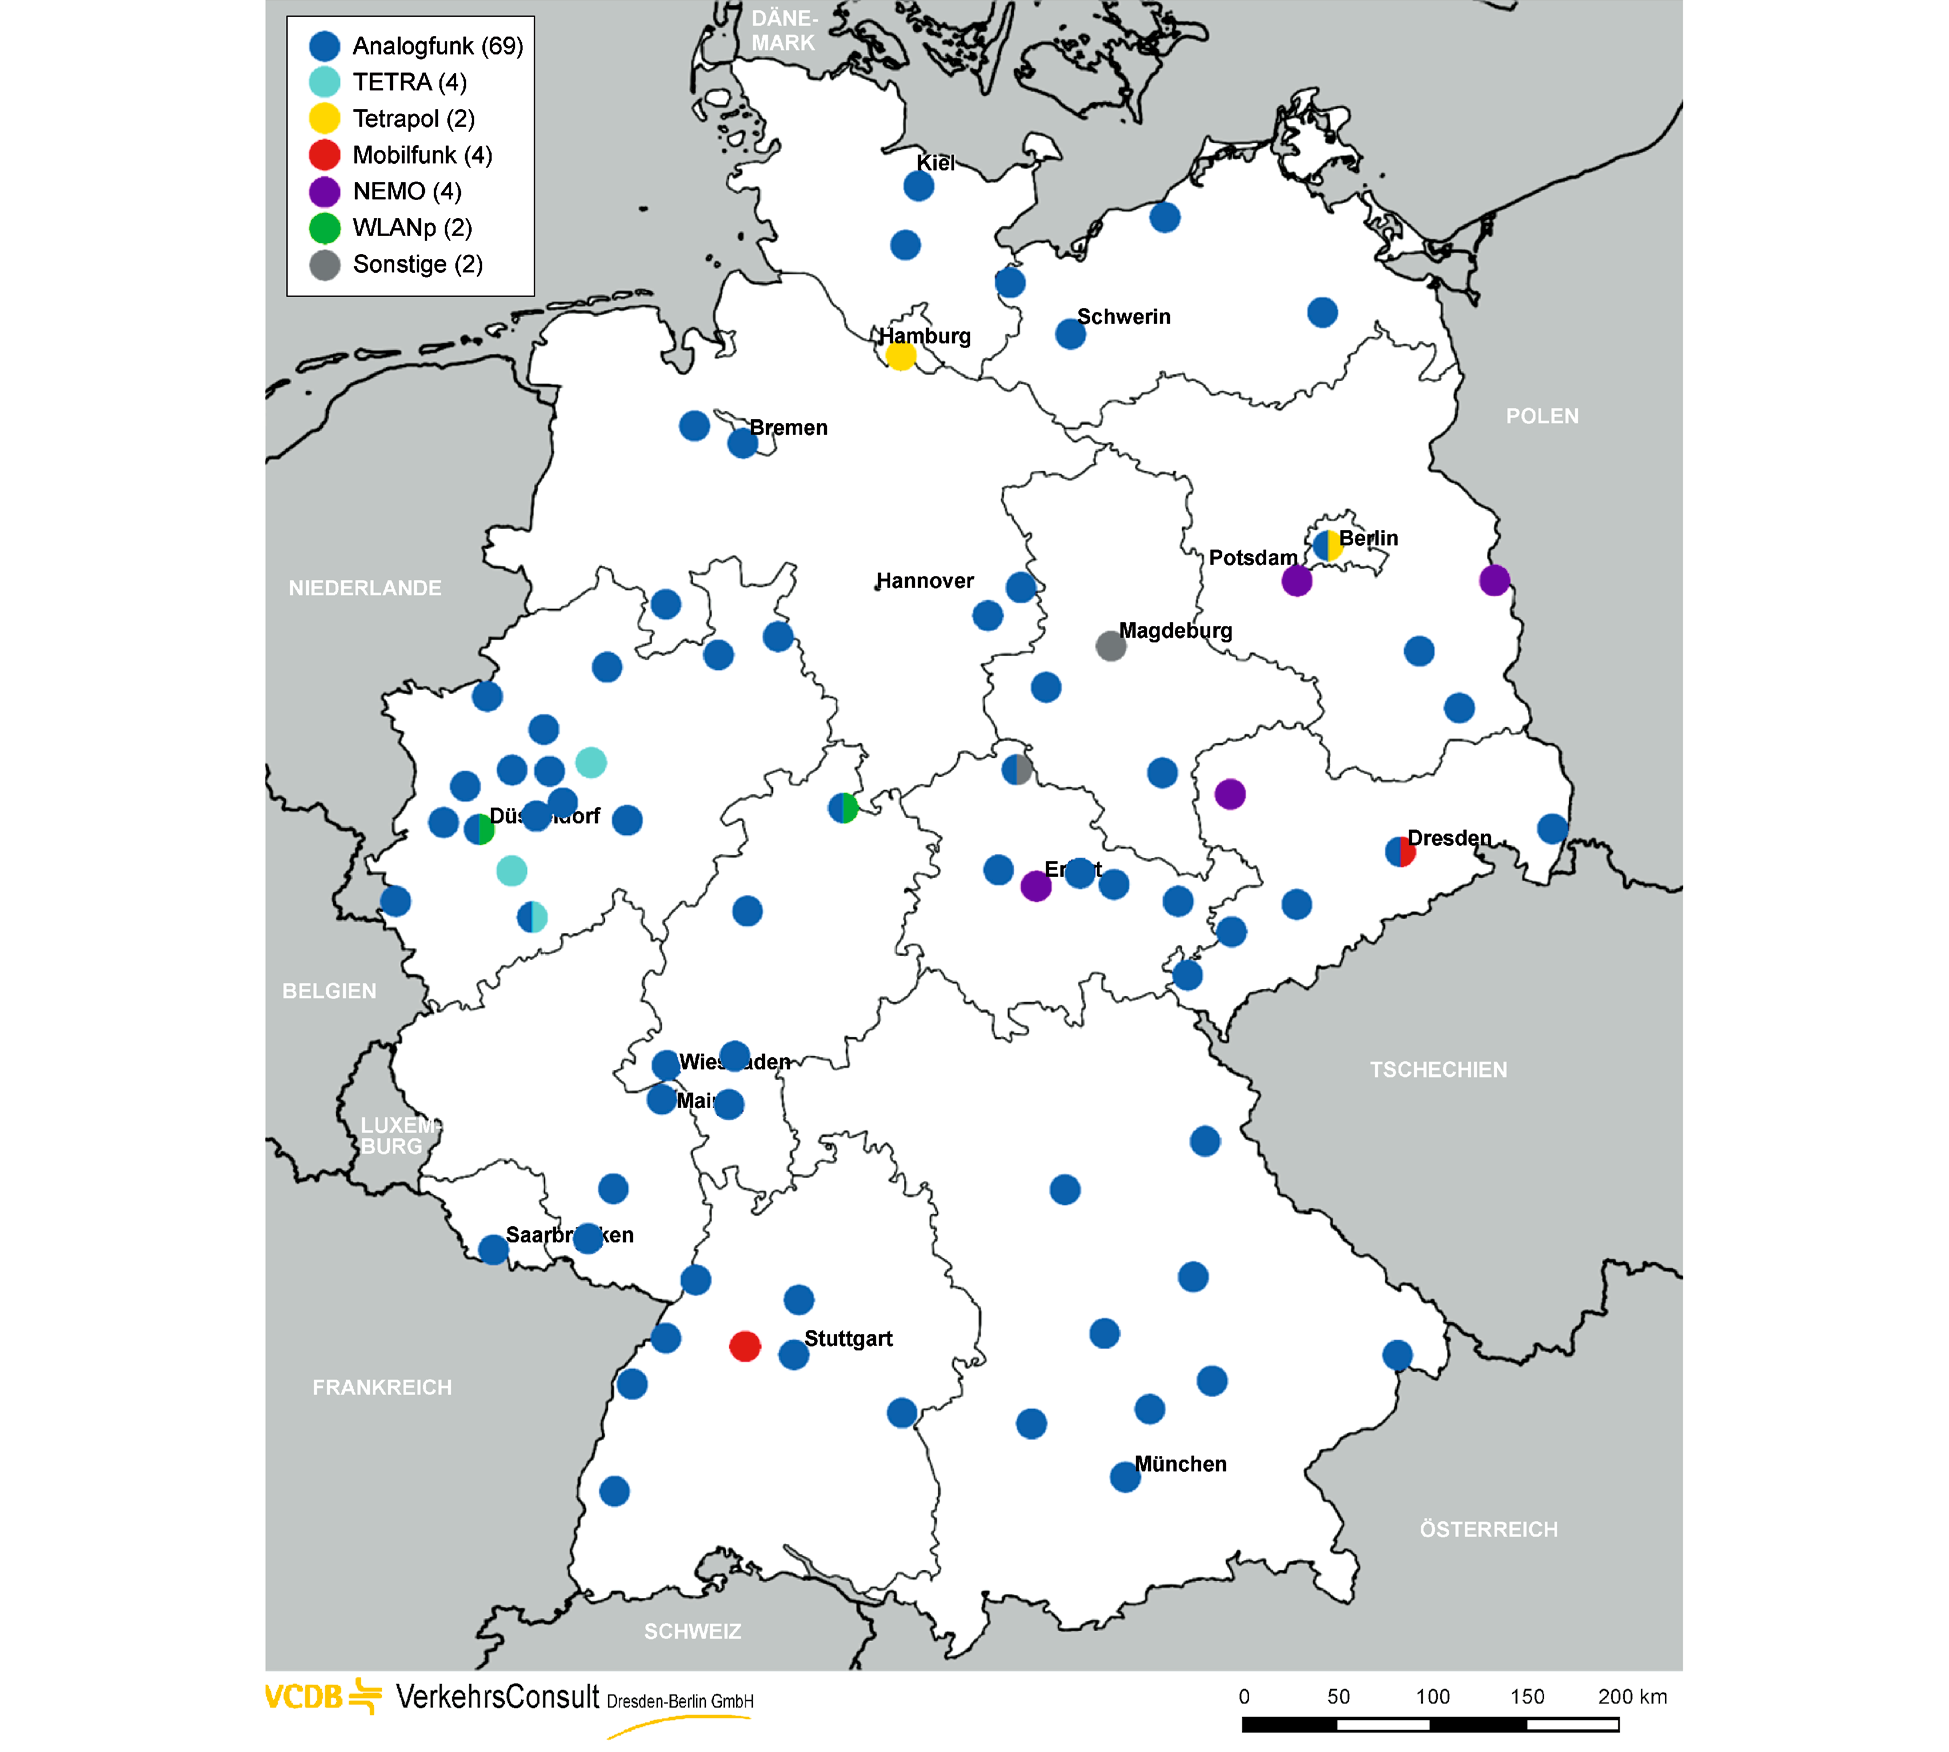
\includegraphics[height=0.8\textheight]{figs/vcdb-map-ampelbeeinflussung.png}
\column{.5\linewidth}
\caption{Map with selected locations which have traffic lights, controlled by public transport. Blue points use the standard we implemented.}
\vspace{0.5cm}
\begin{itemize}
	\item different physical layer protocols described in VDV 426
\end{itemize}
\end{columns}
\end{figure}
\end{frame}

% =================================================

\section{Soul Extrating Information \& Mapping }

%TODO: oxa


% =================================================

\section{Architecture \& Infra }

% =================================================

\begin{frame}
\frametitle{Operating Receivers}
\begin{figure}
\begin{columns}
\column{.5\linewidth}
\begin{center}
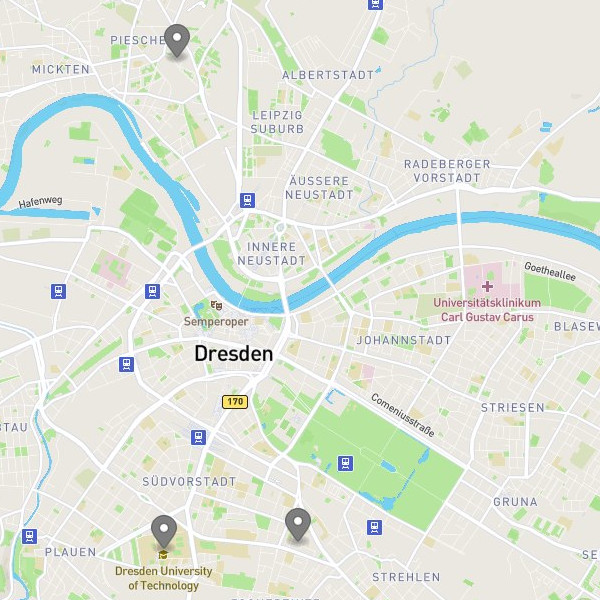
\includegraphics[height=0.7\textheight]{figs/map_dresden.jpg}
\end{center}
\caption{Receivers in Dresden}
\column{.5\linewidth}
\raggedright
\begin{center}
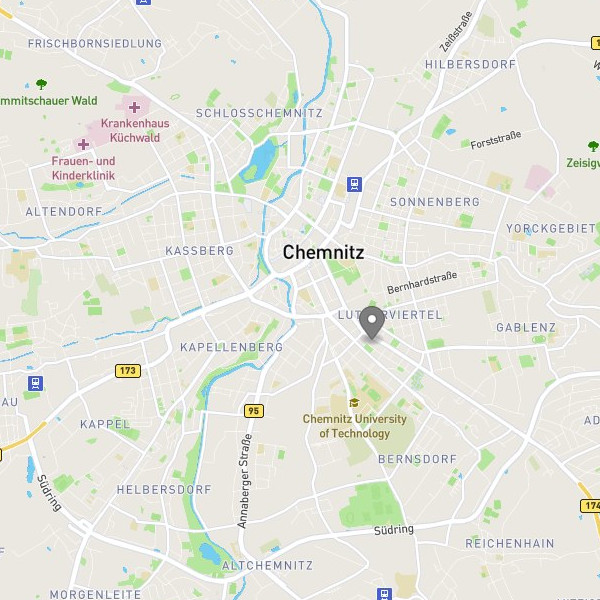
\includegraphics[height=0.6\textheight]{figs/map_chemnitz.jpg}
\end{center}
\caption{Receivers in Chemnitz}

\end{columns}
\end{figure}
\end{frame}

% =================================================

\begin{frame}
\frametitle{Received Data}

\end{frame}

% =================================================

\begin{frame}
\frametitle{Assembeling a Receiver}

\begin{figure}
\begin{columns}
\column{.5\linewidth}
\begin{center}
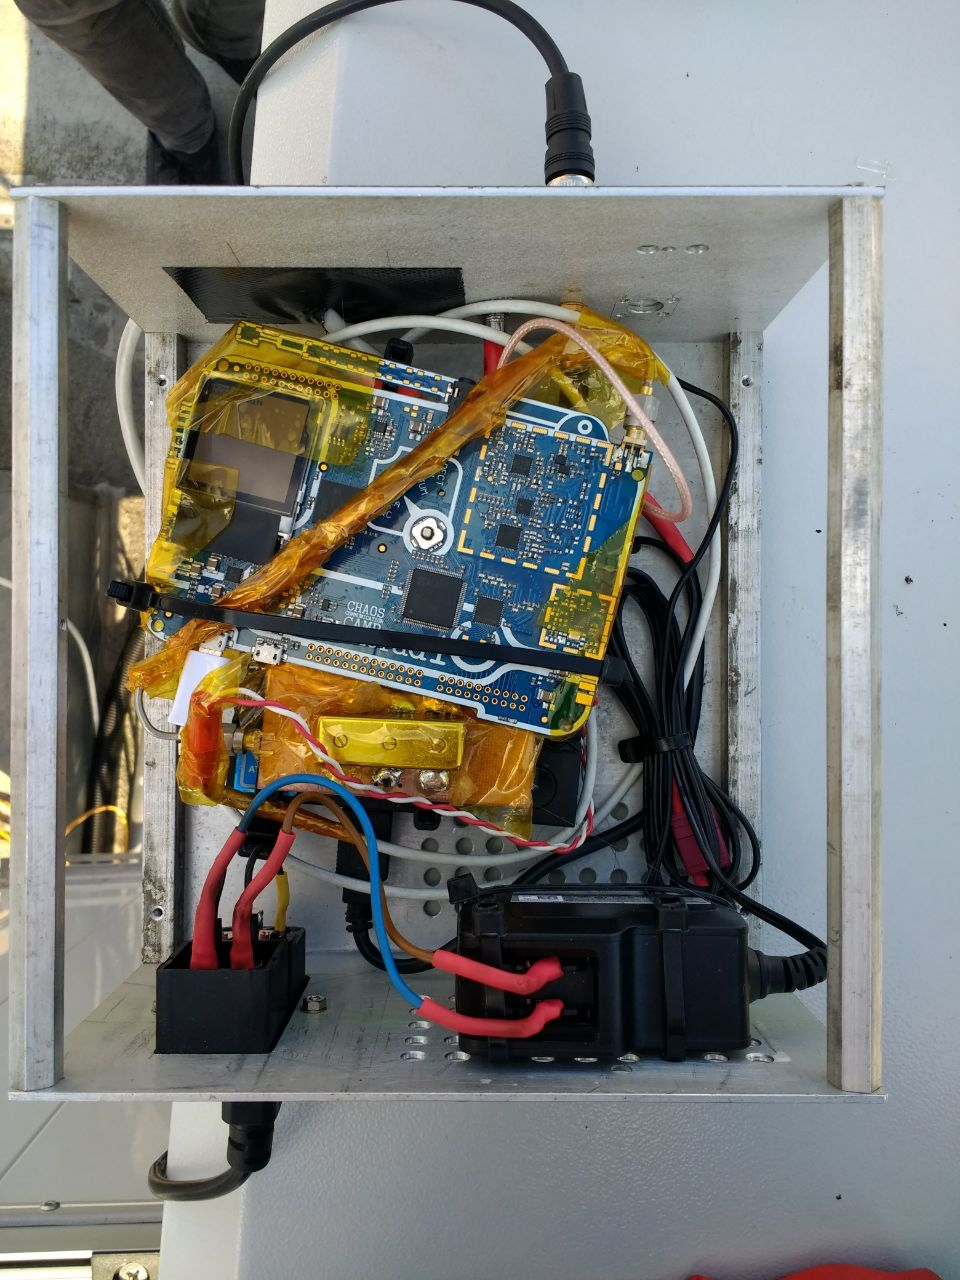
\includegraphics[height=0.7\textheight]{figs/station_barkhausen.jpg}
\end{center}
\column{.5\linewidth}
\raggedright
\caption{Station Barkhausenbau}
\vspace{0.5cm}

\begin{itemize}
	%\item\todo[inline]{make caption allign left}
	%\item\todo[inline]{please provide some details about this station}
  \item VEB powersuply casing (10\$)
  \item Dell Wyse 3040 (30\$)
  \item Rad1o Badge (e.g RTL SDR 30\$)
  \item Hardware Filter (10\$)
  \item Healthy amounts of electric tape
\end{itemize}

$\Rightarrow$ 70\$ - 90\$ per Station

\end{columns}
\end{figure}

\end{frame}

% =================================================

\begin{frame}
\frametitle{Architecture}

% Funnel
% DVB-API
% Clicky-Bunty
% Tracy


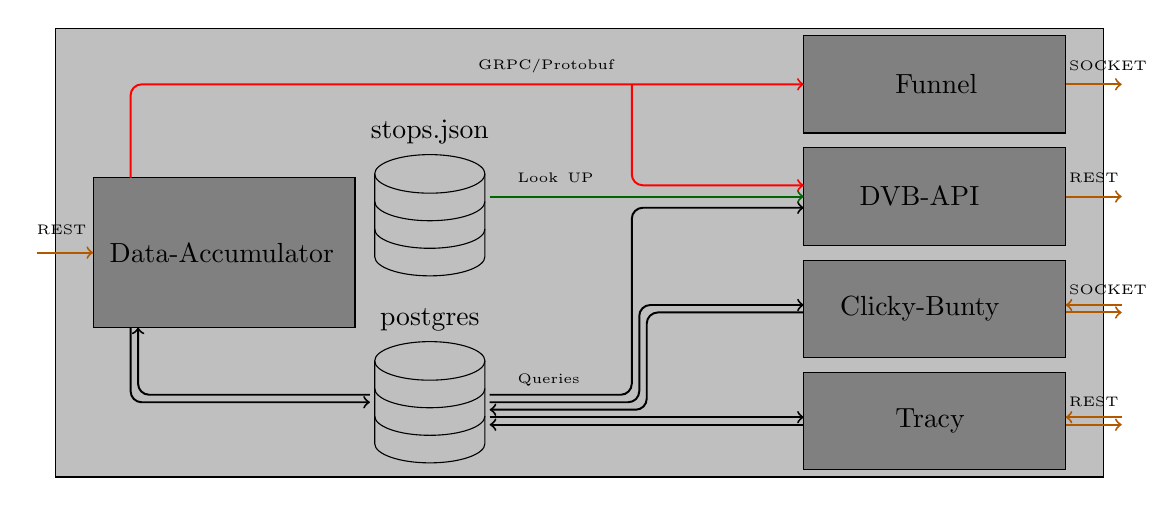
\begin{tikzpicture}[scale=0.95]
  \filldraw[draw=black,fill=lightgray] (5,3) rectangle (19,-3);

  \filldraw[draw=black,fill=gray] (5.5,1) rectangle (9,-1);
  \node[database,label=above:postgres,database radius=0.7cm,database segment height=0.35cm] at (10,-2) {};
  \node[database,label=above:stops.json,database radius=0.7cm,database segment height=0.35cm] at (10,0.5) {};

  % DataAccm <-> Postgres
  \draw[->,rounded corners, line width=0.25mm] (6, -1)  -- (6,-2) -- (9.2,-2);
  \draw[->,rounded corners, line width=0.25mm] (9.2, -1.9)  -- (6.1,-1.9) -- (6.1,-1);

  % User Facing Services
  \filldraw[draw=black,fill=gray] (15,2.9) rectangle (18.5,1.6);
  \filldraw[draw=black,fill=gray] (15,1.4) rectangle (18.5,0.1);
  \filldraw[draw=black,fill=gray] (15,-0.1) rectangle (18.5,-1.4);
  \filldraw[draw=black,fill=gray] (15,-1.6) rectangle (18.5,-2.9);

  % GRPC Arrows
  \draw[->,rounded corners, red, line width=0.25mm] (6, 1)  -- (6,2.25) -- (15,2.25);
  \draw[->,rounded corners, red, line width=0.25mm] (12.7, 2.25)  -- (12.7,0.9) -- (15,0.9);

  % Postgres Arrows
  % Tracy
  \draw[->,rounded corners, line width=0.25mm] (10.8, -2.2)  -- (15,-2.2);
  \draw[->,rounded corners, line width=0.25mm] (15, -2.3)  -- (10.8,-2.3);
  % Clicky-Bunty-Server
  \draw[->,rounded corners, line width=0.25mm] (15, -0.8)  -- (12.9, -0.8) -- (12.9, -2.1) -- (10.8,-2.1);
  \draw[->,rounded corners, line width=0.25mm] (10.8, -2)  -- (12.8, -2) -- (12.8, -0.7) -- (15,-0.7);
  % DVB-API
  \draw[->,rounded corners, line width=0.25mm] (10.8, -1.9)  -- (12.7, -1.9) -- (12.7, 0.6) -- (15, 0.6);

  % Labeling
  \node[text width=3cm] at (7.3,0) {Data-Accumulator};
  \node[text width=1cm] at (16.75,2.25) {Funnel};
  \node[text width=2cm] at (16.8,0.75) {DVB-API};
  \node[text width=2.5cm] at (16.8,-0.75) {Clicky-Bunty};
  \node[text width=1cm] at (16.75,-2.25) {Tracy};

  % Look Ups
  \draw[->,rounded corners, black!60!green, line width=0.25mm] (10.8, 0.75)  -- (15, 0.75);

  % Labeling Arrows
  \node[text width=2cm] at (11.7,2.5) {\tiny GRPC/Protobuf};
  \node[text width=1cm] at (11.7,1) {\tiny Look UP};
  \node[text width=1cm] at (11.7, -1.7) {\tiny Queries};

  \draw[->,rounded corners, black!30!orange, line width=0.25mm] (4.75, 0)  -- (5.5, 0);

  \draw[->,rounded corners, black!30!orange, line width=0.25mm] (18.5, 2.25)  -- (19.25, 2.25);
  \draw[->,rounded corners, black!30!orange, line width=0.25mm] (18.5, 0.75)  -- (19.25, 0.75);


  \draw[->,rounded corners, black!30!orange, line width=0.25mm] (19.25, -0.7)  -- (18.5, -0.7);
  \draw[->,rounded corners, black!30!orange, line width=0.25mm] (18.5, -0.8)  -- (19.25, -0.8);

  \draw[->,rounded corners, black!30!orange, line width=0.25mm] (19.25, -2.2)  -- (18.5, -2.2);
  \draw[->,rounded corners, black!30!orange, line width=0.25mm] (18.5, -2.3)  -- (19.25, -2.3);

  \node[text width=0.1cm] at (4.8,0.3) {\tiny REST};
  \node[text width=0.1cm] at (18.6,1) {\tiny REST};
  \node[text width=0.1cm] at (18.6,-2) {\tiny REST};
  \node[text width=0.1cm] at (18.6,2.5) {\tiny SOCKET};
  \node[text width=0.1cm] at (18.6,-0.5) {\tiny SOCKET};

\end{tikzpicture}

\end{frame}

%TODO: Friendship Ended with Influx

% =================================================

\section{Call for Action}

% =================================================

\begin{frame}
\frametitle{The project is huge you can help !}

\begin{itemize}
  \item Frontend
        \begin{itemize}
          \item \textbf{Tofu}: landing page (TECHNOLOGY OPEN)
          \item \textbf{Tracy}: Mapping Assitent (TECHNOLOGY OPEN)
          \item \textbf{Click}: User + Station Managment (elm-lang)
          \item \textbf{Windshield} Live Map
        \end{itemize}
  \item Setup Stations
  \item Map your City
  \item Find Frequencies
\end{itemize}

\end{frame}

% =================================================

\section{Questions}

\end{document}
